
\documentclass[hyperref={pdfpagelabels=false},ngerman]{beamer}

% stop font warning
\let\Tiny=\tiny
\providecommand\thispdfpagelabel[1]{}

\usepackage[english]{babel}
\usepackage{lmodern}
\usepackage[T1]{fontenc}
\usepackage[utf8]{inputenc}
\usepackage{graphicx,import}
\usepackage{feynmp}
\DeclareGraphicsRule{*}{mps}{*}{} 
\DeclareGraphicsExtensions{.pdf}
\usepackage{amsmath,amssymb,amstext,amsfonts} % mathrsfs
\usepackage{array,booktabs,tabularx}
\usepackage{tikz,tikz-uml,pgf-pie}
\usetikzlibrary{shapes,calc,arrows,positioning,shapes}
\tikzstyle{block} = [rectangle, draw, thick, text width=10em, text centered, minimum height=2em]
\tikzstyle{arrow} = [draw, -latex, thick]
\tikzstyle{arrow2} = [draw, latex-latex, thick]
\tikzstyle{quark}  = [rectangle, draw, fill=yellow, minimum width=2em, text centered, minimum height=2em]
\tikzstyle{lepton} = [rectangle, draw, fill=red!50, minimum width=2em, text centered, minimum height=2em]
\tikzstyle{gauge}  = [circle   , draw, fill=green , minimum size=2em, inner sep=0pt, text centered]
\tikzstyle{scalar} = [diamond  , draw, fill=blue!40, minimum width=2.3em, text centered, minimum height=2.3em, inner sep=0pt]
\tikzstyle{goldstone} = [diamond, draw, dashed, fill=blue!30, minimum width=2.3em, text centered, minimum height=2.3em, inner sep=0pt]
\tikzstyle{squark}   = [diamond, draw, fill=yellow, minimum width=2.3em, text centered, minimum height=2.3em, inner sep=0pt]
\tikzstyle{slepton}  = [diamond, draw, fill=red!50, minimum width=2.3em, text centered, minimum height=2.3em, inner sep=0pt]
\tikzstyle{gaugino}  = [rectangle, draw, fill=green , minimum size=2em, inner sep=0pt, text centered]
\tikzstyle{higgsino} = [rectangle, draw, fill=blue!40  , minimum width=2em, text centered, minimum height=2em]
\tikzstyle{inert}    = [diamond  , draw, fill=teal!80, minimum width=2.3em, text centered, minimum height=2.3em, inner sep=0pt]
\tikzstyle{inertino} = [rectangle, draw, fill=teal!80, minimum width=2em, text centered, minimum height=2em]
\tikzstyle{phantom}  = [rectangle, minimum width=2em, text centered, minimum height=2em]
\usepackage{slashed}
\usepackage{fixltx2e} % textsubscript
\usepackage{multirow}
\usepackage{tcolorbox}
\usepackage{pifont}
\usepackage{xspace}
\usepackage{hyperref}
\hypersetup{colorlinks,linkcolor=,urlcolor=blue}
\usepackage{listings}
\lstset{breaklines=true,
  breakatwhitespace=true,
%  numbers=left,
  numberstyle=\tiny,
  stepnumber=1,
  basicstyle=\ttfamily\footnotesize,
  commentstyle=\ttfamily\color{gray},
  postbreak={\mbox{{$\hookrightarrow$}}\space\space},
  breakindent=10pt,
  breakautoindent=false,
  showspaces=false,
  showstringspaces=false,
  frame=single}

\definecolor{darkgreen}{RGB}{0,176,0}

\newcommand{\cmark}{\ding{51}}%
\newcommand{\xmark}{\ding{55}}%
\newcommand{\fmfvcenter}[1]{\;\vcenter{\hbox{\fmfreuse{#1}}}\;}
\newcommand{\eh}[1]{\,\mathsf{#1}}
\newcommand{\ok}{\textcolor{darkgreen}{\cmark}}
\newcommand{\notok}{\textcolor{red}{\xmark}}
\newcommand{\maybe}{\textcolor{gray}{\cmark}}
\newcommand{\meh}{\textcolor{gray}{\textbf{\huge\lower.1em\hbox{-}}}}
\newcommand{\Lagr}{\mathcal{L}}
\newcommand{\MS}{\ensuremath{M_S}}
\newcommand{\mathi}{\mathsf{i}}
\newcommand{\mycite}[1]{\ensuremath{\text{\textcolor{darkgray}{\tiny [#1]}}}}
\newcommand{\bigcite}[1]{\textcolor{darkgray}{[#1]}}
\newcommand{\dimrep}[1]{\mathbf{#1}}
\newcommand{\dimrepadj}[1]{\mathbf{\overline{#1}}}
\newcommand{\ESSM}{E\textsubscript{6}SSM}
\newcommand{\CESSM}{CE\textsubscript{6}SSM}
\DeclareMathOperator{\tildeRe}{\widetilde Re}
\DeclareMathOperator{\sign}{sign}
\DeclareMathOperator{\re}{Re}
\DeclareMathOperator{\im}{Im}
\renewcommand{\emph}{\textbf}
\newcommand{\dd}{\mathsf{d}}
\newcommand{\myurl}[1]{\href{#1}{#1}}
\newcommand{\Superpot}{\mathcal{W}}
\newcommand{\SuperField}[1]{#1}
\newcommand{\ConjSuperField}[1]{\bar{#1}}
\newcommand{\UY}{\ensuremath{U(1)_{Y}}}
\newcommand{\UN}{\ensuremath{U(1)_{N}}}
\newcommand{\Uem}{\ensuremath{U(1)_\text{em}}}
\newcommand{\SUL}{\ensuremath{SU(2)_\text{L}}}
\newcommand{\SUc}{\ensuremath{SU(3)_\text{c}}}
\newcommand{\SOten}{\ensuremath{{SO(10)}}}
\newcommand{\comma}{,}
\newcommand{\DRbar}{\ensuremath{\overline{\text{DR}}}}
\newcommand{\MSbar}{\ensuremath{\overline{\text{MS}}}}
\newcommand{\SM}{\ensuremath{\text{SM}}}
\newcommand{\MSSM}{\ensuremath{\text{MSSM}}}
\newcommand{\pole}{\ensuremath{\text{pole}}}
\newcommand{\tree}{\ensuremath{\text{tree}}}
\newcommand{\fsstar}{\textbf{*}}
\newcommand{\Zv}{\ensuremath{\backslash\mkern-11.0mu{Z_3}}}
\newcommand{\downrightknickarrow}{\mathrel{\scalebox{1.3}{\rotatebox[origin=c]{180}{$\Lsh$}}}}
\newcommand{\threelinebrace}{$\left. \begin{array}{c} \\ \\ \\ \end{array} \right\rbrace$}
\newcommand{\fivelinebrace}{$\left. \begin{array}{c} \\ \\ \\ \\ \\ \end{array} \right\rbrace$}
\newcommand{\twolinebrace}{$\left. \begin{array}{c} \\ \\ \end{array} \right\rbrace$}
\newcommand{\elevenlinebrace}{$\left. \begin{array}{c} \\ \\ \\ \\ \\ \\ \\ \\ \\ \\ \\ \end{array} \right\rbrace$}
\newcommand{\at}{\alpha_t}
\newcommand{\ab}{\alpha_b}
\newcommand{\atau}{\alpha_\tau}
\newcommand{\as}{\alpha_s}
\newcommand{\SARAH}{\texttt{SARAH}}
\newcommand{\Mathematica}{\texttt{Mathematica}}
\newcommand{\Himalaya}{\texttt{Himalaya}}

% set look of slides
\usetheme{Madrid}
\useoutertheme{default}
\useinnertheme{circles}
\usecolortheme{default}
\beamertemplatenavigationsymbolsempty % keine Navigationselemente
\setbeamersize{text margin left = 1cm, text margin right = 1cm}

% define footer
\makeatletter
\setbeamertemplate{footline}
{
  \hfill\hbox{\insertframenumber{} / \inserttotalframenumber\hspace*{4pt}}%
  \vskip3pt%
}
\makeatother
\usecolortheme{tud}

\title{FlexibleSUSY}

\author[Alexander Voigt]{Alexander Voigt\\[0.5em]{\small In
    collaboration with P.\ Athron, M.\ Bach, D.\ Harries, T.\
    Kwasnitza, J.-h.\ Park, D.\ Stöckinger, J.\ Ziebell}}

\date{GAMBIT webinar, 27.10.2017}

\institute[Aachen]{RWTH Aachen}
\subject{FlexibleSUSY,MSSM,Higgs,FlexibleEFTHiggs}
\keywords{FlexibleSUSY,MSSM,Higgs,FlexibleEFTHiggs}

%%%%%%%%%%%%%%%%%%%%%%%%%%%%%%%%%%%%%%%%%%%%%%%%%%%%%%%%%%%%%%%%%%%%%%%%%%%%%

\begin{document}

%%%%%%%%%%%%%%%%%%%%%%%%%%%%%%%%%%%%%%%%
\begin{frame}[plain]
  \tikz [remember picture,overlay]
  \node at
    ([yshift=1.3cm,xshift=4cm]current page.south)
    {\includegraphics[height=2cm]{images/RWTH_Logo}};
  \titlepage  
\end{frame}

%%%%%%%%%%%%%%%%%%%%%%%%%%%%%%%%%%%%%%%%
\begin{frame}{Contents}
  \tableofcontents
\end{frame}

\section{What is FlexibleSUSY?}

\begin{frame}{What is FlexibleSUSY?}
  \begin{center}
    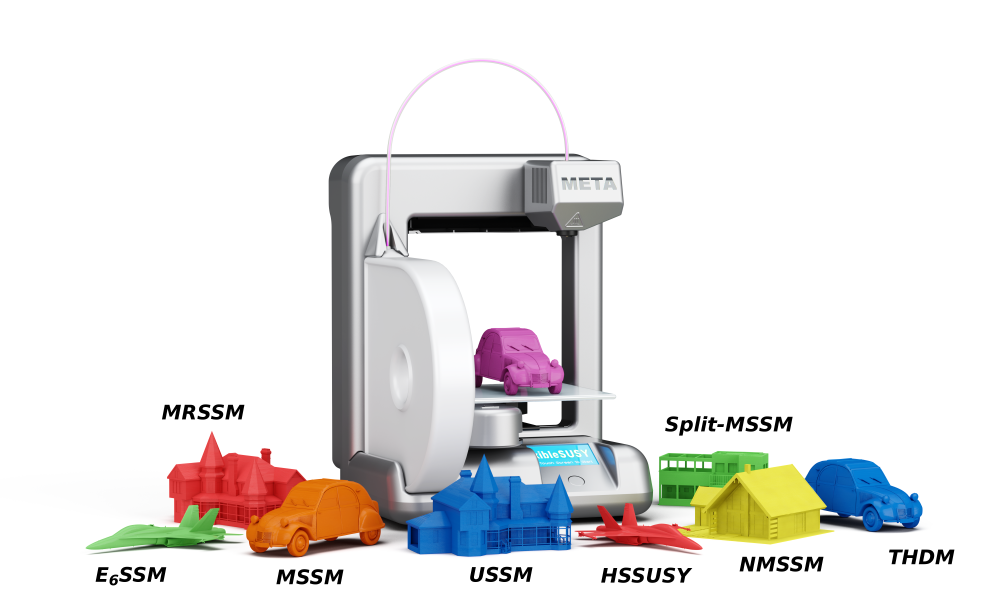
\includegraphics[width=\textwidth]{images/FS.png}
  \end{center}
\end{frame}

\begin{frame}{What is FlexibleSUSY?}
  \begin{center}
    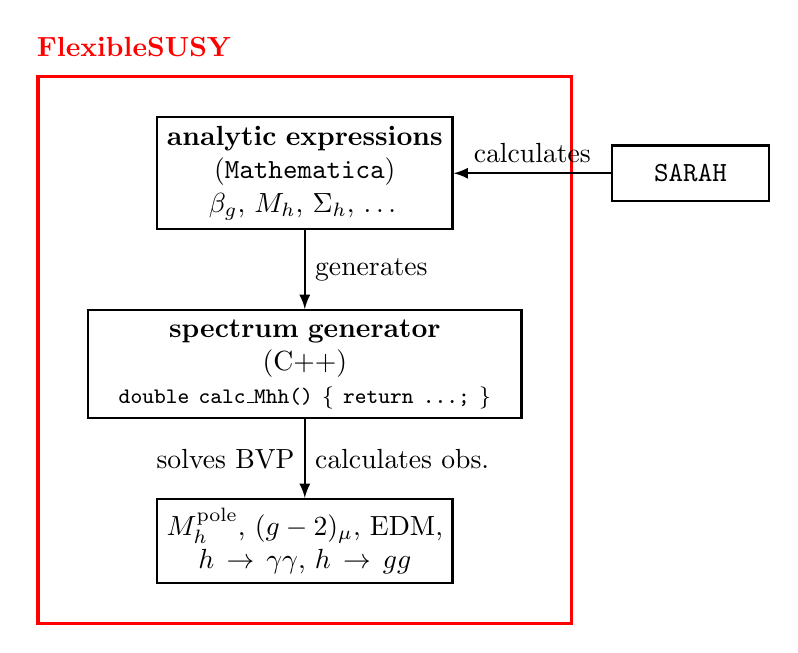
\begin{tikzpicture}
    \node[block] (EXPR) {\textbf{analytic expressions}\\ (\Mathematica)\\ $\beta_g$, $M_h$, $\Sigma_h$, \ldots};
    % \node[block, below = 1cm of EXPR, text width=15em] (FS) {\textbf{spectrum generator}\\ (C++)\\ solves BVP, calculates observables};
    \node[block, below = 1cm of EXPR, text width=15em] (FS) {\textbf{spectrum generator}\\ (C++)\\ \footnotesize{\texttt{double calc\_Mhh() \{ return ...; \}}}};
    \node[block, below = 1cm of FS] (OUT) {$M_h^\pole$, $(g-2)_\mu$, EDM, $h\rightarrow\gamma\gamma$, $h\rightarrow gg$};
    \path[arrow] (EXPR) -- node[right]{generates} (FS);
    \path[arrow] (FS) -- node[right]{calculates obs.} node[left]{solves BVP} (OUT);
    \draw[red,very thick] ($(EXPR.north west)+(-1.5,0.5)$) node(FSname){} rectangle ($(OUT.south east)+(1.5,-0.5)$);
    \node[above right = 0cm and 0cm of FSname.north west] {\textbf{\textcolor{red}{FlexibleSUSY}}};
    \node[block, right = 2cm of EXPR, text width=5em] (SARAH) {\textbf{\SARAH}};
    \path[arrow] (SARAH) -- node[above]{calculates} (EXPR);
    \end{tikzpicture}
  \end{center}
\end{frame}

\begin{frame}{Example: CMSSM}
  BVP
\end{frame}

\section{Features}

\begin{frame}{Features for all models}
  Physics features:
  \begin{itemize}
  \item calculation in the \MSbar/\DRbar\ scheme
  \item real or complex parameters
  \item 2-loop running (RGEs from \SARAH)
  \item 1-loop threshold corrections
  \item 1-loop pole masses (1-loop corrections from \SARAH)
  \item 1-loop $(g-2)_\mu$ + 2-loop leading QED log
  \item 1-loop EDMs for all fundamental fermions
  \item effective couplings $h\rightarrow \gamma\gamma$ and
    $h\rightarrow gg$ at N$^3$LO QCD
  \item 1-loop $M_W$ prediction from $G_F$ + 2-loop SM contributions
  \end{itemize}
  %
  Non-physics features:
  \begin{itemize}
    \item SLHA input/output
    \item \Mathematica\ input/output
    \item SQL database output
    \item modular C++ code
  \end{itemize}
\end{frame}

\begin{frame}{Model-specific features}
  \emph{MSSM:}
  \begin{itemize}
  \item 3-loop running
  \item 2-loop SQCD threshold corrections to $y_t$, $y_b$, $\alpha_s$
  \item 2-loop contributions to $M_{h,H,A}$
  \item 3-loop contributions to $M_h$ (via \Himalaya)
  \end{itemize}
  \emph{NMSSM:}
  \begin{itemize}
  \item 2-loop SQCD threshold corrections to $y_t$, $y_b$, $\alpha_s$
  \item 2-loop contributions to $M_{h,H,A}$
  \end{itemize}
  \emph{SM:}
  \begin{itemize}
  \item 3-loop running
  \item 3-loop QCD threshold corrections to $y_t$, $y_b$, $\alpha_s$
  \item 3-loop contributions to $M_h$
  \item 2-loop threshold corrections to the MSSM (\texttt{HSSUSY})
  \end{itemize}
  \emph{split-MSSM:}
  \begin{itemize}
  \item 2-loop QCD threshold corrections to $y_t$, $y_b$, $\alpha_s$
  \item 3-loop contributions to $M_h$
  \item 2-loop threshold corrections to the MSSM (\texttt{SplitMSSM})
  \end{itemize}
\end{frame}

\section{Supersymmetry and the Higgs sector}

\begin{frame}{Contents}
  \tableofcontents[currentsection]  
\end{frame}

\begin{frame}{Supersymmetry}
  Still an attractive extension of the Standard Model!\\[1em]
  \emph{Features:}
  \begin{itemize}
  \item can predict the SM-like Higgs mass (see later)
  \item gauge coupling unification at $\sim 10^{16}\eh{GeV}$ (due to
    extra matter)
  \item possible connection to super-gravity models and string theory
    (\ESSM, MRSSM)
  \item can explain deviation of $(g-2)_\mu$
  \item can stabilize the electroweak vacuum (see later)
  % \item can solve the hierarchy problem (heavy BSM particles can give
  %   large corrections to the Higgs mass)
  \end{itemize}
  \vspace{1em}
  \emph{Problem:} LHC has not found any SUSY particles so far
  $\Rightarrow$ SUSY particles are probably heavy
\end{frame}

\begin{frame}{Current limits on SUSY particle masses}
  \begin{center}
    \includegraphics[width=\textwidth]{images/ATLAS_SUSY_Summary}
  \end{center}
\end{frame}

\begin{frame}{CP-even Higgs masses in the real MSSM}
  $\left(\im H_d^0, \im H_u^0\right) \overset{\beta}{\rightarrow} (G^0, A)$,
  $\left(\re H_d^0, \re H_u^0\right) \overset{\alpha}{\rightarrow} (h, H)$:
  \begin{align*}
    m_{h,H}^2 = \frac{1}{2} \left[
      m_Z^2 + m_A^2 \mp \sqrt{(m_Z^2 + m_A^2)^2 - 4 m_Z^2 m_A^2 c_{2\beta}^2}
    \right]
  \end{align*}
  If $m_A \gg m_Z$ $\Rightarrow$
  \begin{align*}
    m_h^2 \approx m_Z^2 c_{2\beta}^2
    % = \frac{1}{4} (g_Y^2 + g_2^2) v^2 c_{2\beta}^2
    \leq (91.2 \eh{GeV})^2  \qquad \text{(tree-level)}
  \end{align*}
  $\Rightarrow$ $M_h \approx 125\eh{GeV}$ requires \emph{large loop
    corrections}!
  \begin{align*}
    M_h^2 &= m_h^2 + \Delta m_h^2
    & &\Rightarrow &
    \Delta m_h^2 &\geq (85\eh{GeV})^2
  \end{align*}
  Because of large loop corrections $\Delta m_h^2$:
  \begin{align*}
    \Delta M_h^{\text{theo}} &\gtrsim (1\ldots 2)\eh{GeV} \quad \text{at least!} \\
    \Delta M_h^{\text{exp}} &= 0.24\eh{GeV} \ \ \mycite{PDG-2017}
  \end{align*}
\end{frame}

%%%%%%%%%%%%%%%%%%%%%%%%%%%%%%%%%%%%%%%%

\section{Higgs mass calculation in the MSSM}

\subsection{at fixed loop order}

\begin{frame}{Contents}
  \tableofcontents[
  currentsection,
  currentsubsection,
  subsectionstyle=show/shaded/hide]  
\end{frame}

% Savebox which contains the the Feynman rules
\newsavebox{\feynmanrules}
\sbox{\feynmanrules}{
\begin{fmffile}{Feynman/higgs} % file name and path
  \fmfset{thin}{.8pt}
  \fmfset{wiggly_len}{5mm}
  \fmfset{dash_len}{2.5mm}
  \fmfset{dot_size}{1thick}
  \fmfset{arrow_len}{2.5mm}
  \fmfset{curly_len}{2.5mm}

\begin{fmfgraph*}(60,60)
  \fmfkeep{htop}
  \fmfleft{v1}
  \fmfright{v2}
  \fmf{higgs}{v1,c1}
  \fmf{higgs}{c2,v2}
  \fmf{quark,left,tension=0.5,label=$t$}{c1,c2}
  \fmf{quark,left,tension=0.5}{c2,c1}
\end{fmfgraph*}

\begin{fmfgraph*}(60,60)
  \fmfkeep{hstop}
  \fmfleft{v1}
  \fmfright{v2}
  \fmf{higgs}{v1,c1}
  \fmf{higgs}{c2,v2}
  \fmf{scalar,left,tension=0.5,label=$\tilde{t}_i$}{c1,c2}
  \fmf{scalar,left,tension=0.5}{c2,c1}
\end{fmfgraph*}

\begin{fmfgraph*}(60,60)
  \fmfkeep{hstopA}
  \fmfleft{v1}
  \fmfright{v2}
  \fmf{higgs}{v1,c,v2}
  \fmf{scalar,right,tension=0.8,label=$\tilde{t}_i$}{c,c}
\end{fmfgraph*}

\begin{fmfgraph*}(60,60)
  \fmfkeep{htoptad}
  \fmfleft{v1}
  \fmfright{v2}
  \fmftop{t1}
  \fmf{higgs}{v1,c,v2}
  \fmffreeze
  \fmf{higgs}{c,c1}
  \fmf{quark,right,tension=0.3,label=$t$}{c1,c2}
  \fmf{quark,right,tension=0.3}{c2,c1}
  \fmf{phantom,tension=10}{c2,t1}
\end{fmfgraph*}

\begin{fmfgraph*}(60,60)
  \fmfkeep{hstoptad}
  \fmfleft{v1}
  \fmfright{v2}
  \fmftop{t1}
  \fmf{higgs}{v1,c,v2}
  \fmffreeze
  \fmf{higgs}{c,c1}
  \fmf{scalar,right,tension=0.3,label=$\tilde{t}_i$}{c1,c2}
  \fmf{scalar,right,tension=0.3}{c2,c1}
  \fmf{phantom,tension=10}{c2,t1}
\end{fmfgraph*}
\end{fmffile}
}

\begin{frame}{Fixed loop order calculation}
  Dominant contribution to $M_h$ at the 1-loop level:
  \begin{align*}
    (\Delta m_h^2)^{1L} &= -\Sigma_h^{1L}(p^2) + \frac{t_h^{1L}}{v} \\
    &= \fmfvcenter{htop} + \fmfvcenter{hstop} + \fmfvcenter{hstopA} \\
    &\phantom{={}} + \fmfvcenter{htoptad} + \fmfvcenter{hstoptad} \\
    &\approx \frac{12 m_t^2 y_t^2}{(4\pi)^2} \left(
      \ln\frac{\MS^2}{m_t^2}
      + \frac{X_t^2}{\MS^2}
      - \frac{X_t^4}{12 \MS^4}
    \right) + O(p^2)
  \end{align*}
\end{frame}

\begin{frame}{Summary of fixed loop order calculation}
  Typical order of magnitude of loop contributions (depends on
  parameter scenario):
  \begin{align*}
    M_h &= m_h + \Delta m_h^{1L} + \Delta m_h^{2L} + \Delta m_h^{3L} + \cdots \\
    &\approx [91 + O(20\ldots 30) + O(2\ldots 4) + O(1\ldots 2)] \eh{GeV}
  \end{align*}
  \emph{Advantages:}
  \begin{itemize}
  \item includes logarithmic, non-logarithmic and suppressed terms of
    the order $O(v^2/\MS^2)$ at fixed loop order
  \item precise prediction if $\MS \sim m_t$
  \end{itemize}
  \emph{Problem:}
  \begin{itemize}
  \item large logarithmic corrections, if $\MS \gg m_t$ \\
    $\Rightarrow$ slow convergence of perturbation series \\
    $\Rightarrow$ large theoretical uncertainty, ($1$--$2\eh{GeV}$, or
    more) \\
    $M_h^{\text{exp}} = (125.09 \pm 0.24)\eh{GeV}$
  \end{itemize}
\end{frame}

%%%%%%%%%%%%%%%%%%%%%%%%%%%%%%%%%%%%%%%%

\subsection{in an EFT}

\begin{frame}{Contents}
  \tableofcontents[
  currentsection,
  currentsubsection,
  subsectionstyle=show/shaded/hide]  
\end{frame}

\begin{frame}{Higgs mass calculation in an EFT}
  \emph{Idea:} Integrate out SUSY particles at $\MS$ (expand in $v^2/\MS^2$) \\
  $\Rightarrow$ $\lambda(\MS)$ is fixed by the MSSM \\
  $\Rightarrow$ effectively: separation of scales $\MS$ and $M_t$.
  \begin{center}
    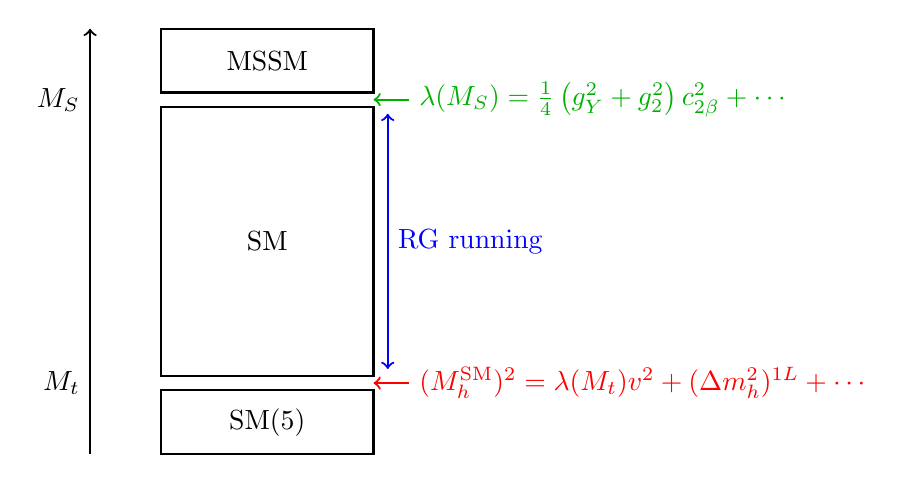
\begin{tikzpicture}[scale=0.9]
      \draw[->, thick] (0,0) -- (0,1) node[left]{$M_t$} -- (0,5) node[left]{$\MS$} -- (0,6);
      \draw[thick] (1,0)   rectangle node{SM(5)} (4,0.9);
      \draw[thick] (1,1.1) rectangle node{SM}    (4,4.9);
      \draw[thick] (1,5.1) rectangle node{MSSM}  (4,6);
      \draw[<-, thick, darkgreen] (4,5) -- (4.5,5) node[right]{$\lambda(\MS) = \frac{1}{4}\left(g_Y^{2} + g_2^2\right) c^2_{2\beta} + \cdots$};
      \draw[<-, thick, red] (4,1) -- (4.5,1) node[right]{$(M_h^\SM)^2 = \lambda(M_t) v^2 + (\Delta m_h^2)^{1L} + \cdots$};
      \draw[<->, thick, blue] (4.2,1.2) -- node[right]{RG running} (4.2,4.8);
    \end{tikzpicture}
  \end{center}
\end{frame}

\begin{frame}{Summary of EFT approach}
  Typical order of magnitude of loop contributions (depends on
  parameter scenario, here $X_t = 0$, $\MS = 20\eh{TeV}$):
  \begin{align*}
    M_h &= m_h + \Delta m_h^{1L} + \Delta m_h^{2L} + \Delta m_h^{3L} + \cdots \\
    % &= \sqrt{\lambda(M_t)} v + \Delta m_h^{1L} + \Delta m_h^{2L} + \cdots \\
    &\approx [O(124) + O(0.5\ldots 1) + O(0.1\ldots 0.2) + O(0.02\ldots 0.04)] \eh{GeV}
    % &= \sqrt{\lambda(\MS)} v + \text{logs} + \Delta m_h^{1L} + \Delta m_h^{2L} + \cdots \\
    % &\approx [O(84) + O(40) + O(0.5\ldots 1) + O(0.1\ldots 0.2)] \eh{GeV}
  \end{align*}
  \emph{Advantages:}
  \begin{itemize}
  \item large logarithmic fixed order loop corrections are avoided
  \item large logarithms $\propto\ln(M_S/M_t)$ are resummed to all orders
  \end{itemize}
  \emph{Disadvantage:} usually terms $O(v^2/M_S^2)$ are neglected \\
  $\Rightarrow$ imprecise when $v \sim \MS$ \\
  $\Rightarrow$ large theoretical uncertainty when $v \sim \MS$
\end{frame}

\begin{frame}{Comparison of fixed-order and EFT approaches}
  \begin{center}
    \includegraphics[width=0.7\textwidth]{{{plots/uncertainties/Mh_MS_TB-5_Xt-0_FO_EFT}}}
  \end{center}
\end{frame}

%%%%%%%%%%%%%%%%%%%%%%%%%%%%%%%%%%%%%%%%

\subsection{in a mixed approach}

\begin{frame}{Contents}
  \tableofcontents[
  currentsection,
  currentsubsection,
  subsectionstyle=show/shaded/hide]  
\end{frame}

\begin{frame}{FlexibleEFTHiggs approach \mycite{arXiv:1609.00371}}
  \emph{Idea:}
  Determine $\lambda(\MS)$ from the condition
  \begin{align*}
    (M_h^2)_{\SM} \equiv \lambda(\MS) v^2 + (\Delta m_h^2)^{1L}_{\SM} \overset{!}{=} (M_h^2)_{\MSSM}\qquad \text{1L, } Q = \MS
  \end{align*}
  \begin{center}
    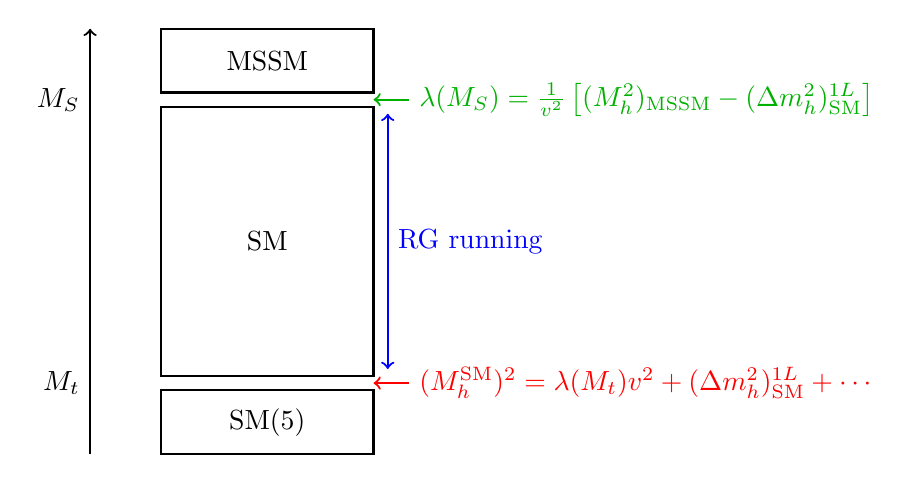
\begin{tikzpicture}[scale=0.9]
      \draw[->, thick] (0,0) -- (0,1) node[left]{$M_t$} -- (0,5) node[left]{$\MS$} -- (0,6);
      \draw[thick] (1,0)   rectangle node{SM(5)} (4,0.9);
      \draw[thick] (1,1.1) rectangle node{SM}    (4,4.9);
      \draw[thick] (1,5.1) rectangle node{MSSM}  (4,6);
      \draw[<-, thick, darkgreen] (4,5) -- (4.5,5) node[right]{$\lambda(\MS) = \frac{1}{v^2}\left[(M_h^2)_{\MSSM} - (\Delta m_h^2)^{1L}_{\SM}\right]$};
      \draw[<-, thick, red] (4,1) -- (4.5,1) node[right]{$(M_h^\SM)^2 = \lambda(M_t) v^2 + (\Delta m_h^2)^{1L}_{\SM} + \cdots$};
      \draw[<->, thick, blue] (4.2,1.2) -- node[right]{RG running} (4.2,4.8);
    \end{tikzpicture}
  \end{center}
\end{frame}

\begin{frame}{Summary FlexibleEFTHiggs approach}
  \begin{align*}
    (M_h^2)_{\SM} &= (M_h^2)_{\MSSM} \qquad \text{1L, } Q = \MS
  \end{align*}
  \emph{Advantages:}
  \begin{itemize}
  \item large logarithms $\propto\ln(M_S/M_t)$ are resummed to all orders
  \item all suppressed terms $O(v^2/\MS^2)$ are incorporated in $\lambda$
  \end{itemize}
  \vspace{1em}
  \textcolor{darkgreen}{$\Rightarrow$ FlexibleEFTHiggs leads to a
    correct Higgs mass prediction at the full 1-loop level (including
    suppressed terms) with additional (N)LL resummation.}\\
  \vspace{1em}
  \emph{Disadvantage:}
  \begin{itemize}
  \item tricky to extend to 2-loop accuracy
  \end{itemize}
\end{frame}

\begin{frame}{Comparison of the three approaches}
  \begin{center}
    \includegraphics[width=0.49\textwidth]{{{plots/uncertainties/Mh_MS_TB-5_Xt-0}}}
    \hfill
    \includegraphics[width=0.49\textwidth]{{{plots/uncertainties/DMh_MS_TB-5_Xt-0}}}
  \end{center}
\end{frame}

%%%%%%%%%%%%%%%%%%%%%%%%%%%%%%%%%%%%%%%%

\section{Summary}

\begin{frame}{Summary}
  \emph{Supersymmetry} is still viable, but LHC continuously excludes
  light SUSY scenarios\\[1em]
  %
  \emph{Approaches to calculate $M_h$:}
  \begin{center}
    \begin{tabular}{lcc}
      \toprule
                               & low $\MS$ & high $\MS$ \\
                               & $\MS \lesssim 2\eh{TeV}$ & $\MS \gtrsim 2\eh{TeV}$ \\
      \midrule
      fixed-order              & \ok       & \notok     \\
      EFT                      & \notok    & \ok        \\
      mixed (FlexibleEFTHiggs) & \ok       & \ok        \\
      \bottomrule
    \end{tabular}
  \end{center}
  %
  \emph{FlexibleEFTHiggs:}
  \begin{itemize}
  \item full NLO + (N)LL resummation
  \item can be applied to \emph{any} BSM model (SUSY or non-SUSY)
  \item can be easily automatized
  \end{itemize}
\end{frame}

%%%%%%%%%%%%%%%%%%%%%%%%%%%%%%%%%%%%%%%%
% backup slides
%%%%%%%%%%%%%%%%%%%%%%%%%%%%%%%%%%%%%%%%

\begin{frame}[noframenumbering]
  \begin{center}
    \Huge Backup
  \end{center}
\end{frame}

%%%%%%%%%%%%%%%%%%%%%%%%%%%%%%%%%%%%%%%%

\begin{frame}[noframenumbering]{Comparison of the three approaches}
  \begin{center}
    \includegraphics[width=0.7\textwidth]{{{plots/FlexibleEFTHiggs-2/scan_Mh_Xt_TB-5_MS-2000}}}
  \end{center}
\end{frame}

%%%%%%%%%%%%%%%%%%%%%%%%%%%%%%%%%%%%%%%%

\begin{frame}[noframenumbering]{FlexibleEFTHiggs -- EFT equivalence}
  \emph{Proof of equivalence:} Start with matching condition:
  \begin{align*}
    (M_h^2)_{\SM} &= (M_h^2)_{\MSSM} \qquad \text{1L, } Q = \MS \\
    \lambda v^2 + (\Delta m_h^2)^{1L}_{\SM} &= (M_h^2)_{\MSSM}
  \end{align*}
  $\Rightarrow$
  \begin{align*}
    \lambda(\MS) &= \frac{1}{v^2} \left[ (M_h^2)_{\MSSM} - (\Delta m_h^2)^{1L}_{\SM} \right] \\
    &= \frac{1}{v^2} \left[
      (m_h^2)_{\MSSM} + (\Delta m_h^2)^{1L}_{\MSSM} - (\Delta m_h^2)^{1L}_{\SM}
    \right]
  \end{align*}
  Now insert $(m_h^2)_{\MSSM}$ and $(\Delta m_h^2)^{1L}_{\MSSM}$ \ldots
\end{frame}

\begin{frame}[noframenumbering]{FlexibleEFTHiggs -- EFT equivalence}
  Inserting \textcolor{darkgreen}{$(m_h^2)_{\MSSM}$} and
  \textcolor{red}{$(\Delta m_h^2)^{1L}_{\MSSM}$} for $X_t = 0$:
  \begin{align*}
    \lambda(\MS) &=
    \frac{1}{v^2} \Bigg[
      \textcolor{darkgreen}{
      \frac{1}{4}(g_Y^2 + g_2^2) v^2 c_{2\beta}^2} \\
      &\quad\qquad \textcolor{red}{ + \frac{c_{\alpha}^2}{s_{\beta}^2} (\Delta m_h^2)^{1L}_{\SM}
        - \frac{c_{\alpha}^2}{s_{\beta}^2} \frac{12 (y_t^{\SM})^2 m_t^2}{(4\pi)^2}
      B_0(m_h^2,\MS^2,\MS^2) } \\
      &\quad\qquad - (\Delta m_h^2)^{1L}_{\SM}
    \Bigg]
  \end{align*}
  Now go to the decoupling limit $c_{\alpha}^2/s_{\beta}^2\rightarrow
  1$ \ldots
\end{frame}

\begin{frame}[noframenumbering]{FlexibleEFTHiggs -- EFT equivalence}
  In the decoupling limit $c_{\alpha}^2/s_{\beta}^2\rightarrow 1$:
  \begin{align*}
    \lambda(\MS) &=
    \frac{1}{4}(g_Y^2 + g_2^2) c_{2\beta}^2
    - 12 \frac{m_t^2 (y_t^{\SM})^2}{(4\pi)^2 v^2} B_0(m_h^2,\MS^2,\MS^2) \\
    &= \frac{1}{4} (g_Y^2 + g_2^2) c_{2\beta}^2
    - 12 \frac{m_t^2 (y_t^\SM)^2}{(4\pi)^2 v^2} \Bigg[ 
    -\log\frac{\MS^2}{Q^2} + \frac{m_h^2}{6\MS^2} + O\Big(\frac{m_h^4}{\MS^4}\Big)
    \Bigg] \\
    &= \frac{1}{4} (g_Y^2 + g_2^2) c_{2\beta}^2
    + 12 \frac{m_t^2 (y_t^\SM)^2}{(4\pi)^2 v^2} \Bigg[ 
    \log\frac{\MS^2}{Q^2} \Bigg] + O\Big(\frac{v^2}{\MS^2}\Big) \\
    &= \lambda^{\text{EFT,tree}} + \Delta\lambda^{\text{EFT},1L} + O\Big(\frac{v^2}{\MS^2}\Big)
  \end{align*}
  In the decoupling limit $\lambda(\MS)$ in the FlexibleEFTHiggs
  approach is equivalent to the EFT approach at 1-loop, up to
  suppressed terms $O(v^2/\MS^2)$
\end{frame}

%%%%%%%%%%%%%%%%%%%%%%%%%%%%%%%%%%%%%%%%

\begin{frame}[noframenumbering]{Higgs mass uncertainty estimate}
  \emph{fixed-order:}
  \begin{itemize}
  \item $|M_h^{2L}(Q_\pole = \MS/2) - M_h^{2L}(Q_\pole = 2\MS)|$
  \item $|M_h^{2L}(y_t^{1L}) - M_h^{2L}(y_t^{2L})|$
  \end{itemize}
  \emph{EFT (SUSYHD):}
  \begin{itemize}
  \item $|M_h^{2L}(Q_\pole = M_t/2) - M_h^{2L}(Q_\pole = 2M_t)|$
  \item $|M_h^{2L}(y_t^{2L}) - M_h^{2L}(y_t^{3L})|$
  \item $|M_h^{2L}(Q_{\text{match}} = \MS/2) - M_h^{2L}(Q_{\text{match}} = 2\MS)|$
  \item $|M_h^{2L} - M_h^{2L}(\lambda \rightarrow \lambda(1 + v^2/\MS^2))|$
  \end{itemize}
  \emph{FlexibleEFTHiggs:}
  \begin{itemize}
  \item $|M_h^{2L}(Q_\pole = M_t/2) - M_h^{2L}(Q_\pole = 2M_t)|$
  \item $|M_h^{2L}(y_t^{2L}) - M_h^{2L}(y_t^{3L})|$
  \item $|M_h^{2L}(Q_{\text{match}} = \MS/2) - M_h^{2L}(Q_{\text{match}} = 2\MS)|$
  \end{itemize}
\end{frame}

%%%%%%%%%%%%%%%%%%%%%%%%%%%%%%%%%%%%%%%%

\begin{frame}[noframenumbering]{Incorrect 2L logs in original FlexibleEFTHiggs-1L}
  Matching condition:
  \begin{align*}
    \lambda &\leftarrow \frac{1}{v^2} \left[
      (m_h^\SM)^2 + (M_h^\text{MSSM})^2 - (M_h^\SM)^2
    \right]
  \end{align*}
  Expansion of momentum iteration up to 1L level:
  \begin{align*}
    \lambda &= \frac{1}{v^2} \Big[
      (m_h^\MSSM)^2
      + \Delta m_{h,\MSSM}^2
      - \Delta m_{h,\SM}^2
      + O(\hbar^2)
    \Big]
  \end{align*}
  with
  \begin{align*}
    \Delta m_{h,\MSSM}^2 &= -\Sigma^{1L}_{\MSSM} + t_{\MSSM}^{1L}/v_\MSSM \\
    \Delta m_{h,\SM}^2 &= -\Sigma^{1L}_{\SM} + t^{1L}_{\SM}/v_\SM
  \end{align*}
\end{frame}

\begin{frame}[noframenumbering]{Incorrect 2L logs in original FlexibleEFTHiggs-1L}
  \emph{Problem:} $y_t^{\MSSM} = y_t^\SM/s_\beta [1 + O(\hbar)] $\\
  $\Rightarrow$
  \begin{align*}
    \Delta m_{h,\MSSM}^2 - \Delta m_{h,\SM}^2 &\propto
    \hbar \Bigg[ (y_t^\MSSM s_\beta)^4 \log\frac{m_t}{M_S} - (y_t^\SM)^4 \log\frac{m_t}{M_S}\Bigg] \\
    &= \hbar \Bigg[0\ + \propto \hbar y_t^4 \log\frac{m_t}{M_S} + O(\hbar^2) \Bigg] \\
    &= O(\hbar^2 y_t^4 \log\frac{m_t}{M_S})
  \end{align*}
  $\Rightarrow$\\
  incorrect 2L logs remain in FlexibleEFTHiggs-1L
\end{frame}

\end{document}
